\documentclass[11pt,a4paper]{article}

\usepackage[utf8]{inputenc}
\usepackage[T1]{fontenc}
\usepackage[english]{babel}
\usepackage{lmodern}

\usepackage{geometry}
\geometry{
    top=2.5cm,
    bottom=2.5cm,
    left=2.5cm,
    right=2.5cm
}

\usepackage{amsmath,amssymb}
\usepackage{booktabs}
\usepackage{array}
\usepackage{graphicx}
\usepackage{listings}
\usepackage{xcolor}
\usepackage{fancyhdr}
\usepackage{hyperref}

\pagestyle{fancy}
\fancyhf{}
\rhead{\textit{Practical 2: Working with Data}}
\lhead{\textit{Data Science --- ETSINF (UPV)}}
\cfoot{\thepage}

\lstset{
    language=R,
    basicstyle=\ttfamily\footnotesize,
    keywordstyle=\color{blue}\bfseries,
    commentstyle=\color{gray}\itshape,
    stringstyle=\color{teal},
    numbers=none,
    frame=lines,
    breaklines=true,
    breakatwhitespace=true,
    showstringspaces=false,
    captionpos=b,
    tabsize=2
}

\title{\textbf{Practical 2: Working with Data}\\[0.4ex] \Large Data Science --- Academic Lab Report}
\author{\textbf{Enrique Sopeña} \\ 
Escola Tècnica Superior d'Enginyeria Informàtica (ETSINF) \\ 
Universitat Politècnica de València}
\date{\today}

\begin{document}

\maketitle

\begin{abstract}
    This report documents the implementation and experimental evaluation of Practical 2 (\textit{Working with data}) in R. The study covers end-to-end data manipulation procedures across standard statistical datasets (\texttt{titanic.csv}, \texttt{cars.csv}, \texttt{airquality.csv}, \texttt{sales.txt}, and relational customer data). Key techniques analyzed include exploratory data inspection, graphic customization, dataset mutation and sorting, conditional data imputation and discretization (equal-width vs.\ quantile binning), date arithmetic, frequency de-aggregation, correlation analysis, simple and stratified sampling, multi-level aggregation, and relational table joining.
\end{abstract}

\vspace{1em}
\hrule
\vspace{1em}

\section{Exercise 1: Inspection of Data}

\subsection{Objective and Commands}
The \texttt{titanic.csv} dataset contains historical survival records from the Titanic disaster. The dataset is ingested using \texttt{read.csv()}, its schema is inspected, the redundant indexing column \texttt{X} is pruned using \texttt{subset()}, and variable properties are evaluated through structural inspection.

\begin{lstlisting}
# Ingestion and redundant index removal
titanic <- read.csv("titanic.csv", header = TRUE, sep = ",")
names(titanic)
titanic <- subset(titanic, select = -X)

# Structural and statistical inspection
head(titanic)
summary(titanic)
str(titanic)
\end{lstlisting}

\subsection{Outputs and Console Verification}
\begin{lstlisting}[language={}]
> names(titanic)
[1] "X"        "Class"    "Sex"      "Age"      "Survived" "Freq"    

> head(titanic)
  Class    Sex   Age Survived Freq
1   1st   Male Child       No    0
2   2nd   Male Child       No    0
3   3rd   Male Child       No   35
4  Crew   Male Child       No    0
5   1st Female Child       No    0
6   2nd Female Child       No    0

> summary(titanic)
    Class               Sex                Age              Survived        
 Length:32          Length:32          Length:32          Length:32         
 Class :character   Class :character   Class :character   Class :character  
 Mode  :character   Mode  :character   Mode  :character   Mode  :character  
      Freq       
 Min.   :  0.00  
 1st Qu.:  0.75  
 Median : 13.50  
 Mean   : 68.78  
 3rd Qu.: 77.00  
 Max.   :670.00  
\end{lstlisting}

\subsection{Discussion: Variable Types Identification}
\begin{itemize}
    \item \textbf{Quantitative Variables:} The only quantitative variable in the dataset is \texttt{Freq} (integer). It represents the absolute count of individuals sharing a specific demographic profile. In \texttt{summary()}, quantitative variables are identified by the presence of continuous statistical metrics (minimum, median, mean, quartiles, and maximum). In \texttt{str()}, it is typed as \texttt{int}.
    \item \textbf{Categorical Variables:} \texttt{Class} (1st, 2nd, 3rd, Crew), \texttt{Sex} (Male, Female), \texttt{Age} (Child, Adult), and \texttt{Survived} (No, Yes) are nominal/ordinal categorical attributes. They represent discrete non-continuous modalities and are typed as \texttt{character} or \texttt{factor} without summary distribution statistics.
\end{itemize}

% -------------------------------------------------------------
\section{Exercise 2: Working with Basic Graphics}

\subsection{Objective and Commands}
The \texttt{cars.csv} dataset records automobile speed (\texttt{speed} in mph) and stopping distance (\texttt{dist} in ft). Basic exploratory visualizations (scatter plots and frequency histograms) are constructed and stylized with distinct color palettes, informative axis labels, and exported directly to PDF vector format.

\begin{lstlisting}
cars <- read.csv("cars.csv", header = TRUE, sep = ",")
if ("X" %in% colnames(cars)) cars <- subset(cars, select = -X)

# Customized Graphics exported to PDF
pdf("plot_cars_scatter.pdf")
plot(cars$speed, cars$dist,
     main = "Stopping Distance vs Speed",
     xlab = "Speed (mph)", ylab = "Stopping Distance (ft)",
     col = "darkblue", pch = 19)
dev.off()

pdf("plot_cars_hist_dist.pdf")
hist(cars$dist, main = "Distribution of Stopping Distance",
     xlab = "Stopping Distance (ft)", ylab = "Frequency",
     col = "steelblue", border = "white")
dev.off()

pdf("plot_cars_hist_speed.pdf")
hist(cars$speed, main = "Distribution of Speed",
     xlab = "Speed (mph)", ylab = "Frequency",
     col = "coral", border = "white")
dev.off()
\end{lstlisting}

\subsection{Visual Inspection}
\begin{figure}[htbp]
    \centering
    \begin{minipage}{0.32\textwidth}
        \centering
        \includegraphics[width=\textwidth]{../dataset/plot_cars_scatter.pdf}
        \caption{Distance vs.\ Speed}
    \end{minipage}\hfill
    \begin{minipage}{0.32\textwidth}
        \centering
        \includegraphics[width=\textwidth]{../dataset/plot_cars_hist_dist.pdf}
        \caption{Distance Histogram}
    \end{minipage}\hfill
    \begin{minipage}{0.32\textwidth}
        \centering
        \includegraphics[width=\textwidth]{../dataset/plot_cars_hist_speed.pdf}
        \caption{Speed Histogram}
    \end{minipage}
\end{figure}

The scatter plot highlights an upward curvilinear association between travel velocity and braking displacement. The distance histogram reveals a right-skewed distribution, whereas automobile speed displays an approximately symmetric profile.

% -------------------------------------------------------------
\section{Exercise 3: Transformations of Variables and Datasets}

\subsection{Objective and Commands}
The base \texttt{cars} data frame is augmented with two newly acquired observations: $(\text{speed}=21, \text{dist}=47)$ and $(\text{speed}=34, \text{dist}=87)$. The combined data frame is subsequently ordered along the \texttt{speed} dimension using direct array indexing with \texttt{order()} and contextual scope evaluation with \texttt{with()}.

\begin{lstlisting}
# Construct auxiliary data frame
new_cars <- data.frame(speed = c(21, 34), dist = c(47, 87))

# Row-bind datasets
cars_extended <- rbind(cars, new_cars)

# Sort ascending by speed
cars_sorted1 <- cars_extended[order(cars_extended$speed), ]
cars_sorted2 <- cars_extended[with(cars_extended, order(speed)), ]
identical(cars_sorted1, cars_sorted2)
\end{lstlisting}

\subsection{Outputs}
\begin{lstlisting}[language={}]
> tail(cars_extended)
   speed dist
47    24   92
48    24   93
49    24  120
50    25   85
51    21   47
52    34   87

> identical(cars_sorted1, cars_sorted2)
[1] TRUE

> tail(cars_sorted1, 10)
   speed dist
43    20   64
51    21   47
44    22   66
45    23   54
46    24   70
47    24   92
48    24   93
49    24  120
50    25   85
52    34   87
\end{lstlisting}
Both sorting methods achieve identical permutations. In the final sorted structure, observation 51 ($\text{speed}=21$) is positioned between records with speeds 20 and 22, while observation 52 ($\text{speed}=34$) represents the maximum boundary.

% -------------------------------------------------------------
\section{Exercise 4: Data Manipulation}

\subsection{Objective and Commands}
Exploratory slicing, missing-value profiling, and conditional aggregation are performed on \texttt{airquality.csv}.

\begin{lstlisting}
air <- read.csv("airquality.csv", header = TRUE, sep = ",")
if ("X" %in% colnames(air)) air <- subset(air, select = -X)

# 1. First 2 rows
head(air, 2)

# 2. Number of observations
nrow(air)

# 3. Ozone value at row 40
air[40, "Ozone"]

# 4. Total missing values in Ozone
sum(is.na(air$Ozone))

# 5. Ozone sample mean excluding NA
mean(air$Ozone, na.rm = TRUE)

# 6. Subset: Ozone > 31 & Temp > 90; compute Solar.R mean
subset_air <- subset(air, Ozone > 31 & Temp > 90)
mean(subset_air$Solar.R, na.rm = TRUE)
\end{lstlisting}

\subsection{Console Results}
\begin{lstlisting}[language={}]
> head(air, 2)
  Ozone Solar.R Wind Temp Month Day
1    41     190  7.4   67     5   1
2    36     118  8.0   72     5   2

> nrow(air)
[1] 153

> air[40, "Ozone"]
[1] 71

> sum(is.na(air$Ozone))
[1] 37

> mean(air$Ozone, na.rm = TRUE)
[1] 42.12931

> mean(subset_air$Solar.R, na.rm = TRUE)
[1] 212.8
\end{lstlisting}
\begin{itemize}
    \item Row 40 reports an Ozone concentration of \textbf{71} ppb.
    \item Exactly \textbf{37} records out of 153 are unobserved (\texttt{NA}) in the \texttt{Ozone} column ($24.18\%$).
    \item The unweighted mean Ozone level is $\bar{x} \approx 42.13$ ppb.
    \item When conditioning on high-temperature, high-ozone episodes ($\text{Ozone} > 31 \land \text{Temp} > 90$), mean solar radiation is $\bar{x}_{\text{Solar.R}} = 212.8$ langleys.
\end{itemize}

% -------------------------------------------------------------
\section{Exercise 5: Data Transformation (Discretization and Dates)}

\subsection{Objective and Commands}
Continuous features are discretized using two core strategies: equal-width partitioning via \texttt{cut()} and equal-frequency (quantile) binning via sample quantiles, explicitly allocating missing entries to a dedicated level (\texttt{binNA}). A sequential elapsed-time metric \texttt{AbsDay} is constructed from calendar attributes.

\begin{lstlisting}
# 5.1 Discretise Ozone into 5 equal-width bins + binNA
ozone_cut <- cut(air$Ozone, breaks = 5, labels = paste0("bin", 1:5), include.lowest = TRUE)
air$Ozone_bin <- as.character(ozone_cut)
air$Ozone_bin[is.na(air$Ozone_bin)] <- "binNA"
air$Ozone_bin <- factor(air$Ozone_bin, levels = c(paste0("bin", 1:5), "binNA"))

# 5.2 Discretise Solar.R into 4 equal-size (quantile) bins + binNA
q_solar <- quantile(air$Solar.R, probs = seq(0, 1, 0.25), na.rm = TRUE)
solar_cut <- cut(air$Solar.R, breaks = q_solar, labels = paste0("bin", 1:4), include.lowest = TRUE)
air$Solar_bin <- as.character(solar_cut)
air$Solar_bin[is.na(air$Solar_bin)] <- "binNA"
air$Solar_bin <- factor(air$Solar_bin, levels = c(paste0("bin", 1:4), "binNA"))

# 5.3 Elapsed calendar days from reference date (1973-05-01)
current_dates <- as.Date(paste(1973, air$Month, air$Day, sep = "-"))
air$AbsDay <- as.numeric(current_dates - as.Date("1973-05-01"))
\end{lstlisting}

\subsection{Outputs and Empirical Distributions}
\begin{lstlisting}[language={}]
> table(air$Ozone_bin)
 bin1  bin2  bin3  bin4  bin5 binNA 
   62    29    18     5     2    37 

> table(air$Solar_bin)
 bin1  bin2  bin3  bin4 binNA 
   37    36    36    37     7 
\end{lstlisting}
\begin{itemize}
    \item \textbf{Equal-width Partitioning (\texttt{Ozone}):} Divides the range into uniform intervals. Because ozone values exhibit positive skewness, the majority of observations are clustered in \texttt{bin1} ($n=62$) and \texttt{bin2} ($n=29$), while upper bins are sparsely populated.
    \item \textbf{Equal-size Partitioning (\texttt{Solar.R}):} Quantile boundaries guarantee an equitable observation balance ($\approx 36$--$37$ records per active bin) alongside the 7 unrecorded instances in \texttt{binNA}.
    \item \textbf{Elapsed Day Count (\texttt{AbsDay}):} Spans values from $0$ (May 1st) to $152$ (September 30th), mapping 153 consecutive temporal indices across the summer monitoring campaign.
\end{itemize}

% -------------------------------------------------------------
\section{Exercise 6: Data Transformation (Titanic Frequency De-aggregation)}

\subsection{Objective and Commands}
Ordinal categorization is mapped to numerical ranks ($\text{3rd}=1, \text{2nd}=2, \text{1st}=3, \text{Crew}=4$). The aggregated contingency table is expanded into an individual-level data frame (\texttt{titanic2}) by replicating rows according to \texttt{Freq}.

\begin{lstlisting}
# Numerise class attribute
class_mapping <- c("3rd" = 1, "2nd" = 2, "1st" = 3, "Crew" = 4)
titanic$Class_num <- class_mapping[as.character(titanic$Class)]

# De-aggregate contingency data frame using rep() and Freq
titanic2 <- titanic[rep(seq_len(nrow(titanic)), titanic$Freq), ]
titanic2 <- subset(titanic2, select = -Freq)
nrow(titanic2)

# Graphical comparison
pdf("plot_titanic_original.pdf", width = 7, height = 5)
plot(titanic, main = "Original Titanic (Aggregated Structure)")
dev.off()

pdf("plot_titanic2_individual.pdf", width = 7, height = 5)
plot(as.data.frame(unclass(titanic2), stringsAsFactors = TRUE),
     main = "De-aggregated Titanic (Individual Records)")
dev.off()
\end{lstlisting}

\subsection{Outputs and Comparative Discussion}
\begin{lstlisting}[language={}]
> table(titanic$Class, titanic$Class_num)
       1 2 3 4
  1st  0 0 8 0
  2nd  0 8 0 0
  3rd  8 0 0 0
  Crew 0 0 0 8

> nrow(titanic2)
[1] 2201
\end{lstlisting}
\begin{figure}[htbp]
    \centering
    \begin{minipage}{0.48\textwidth}
        \centering
        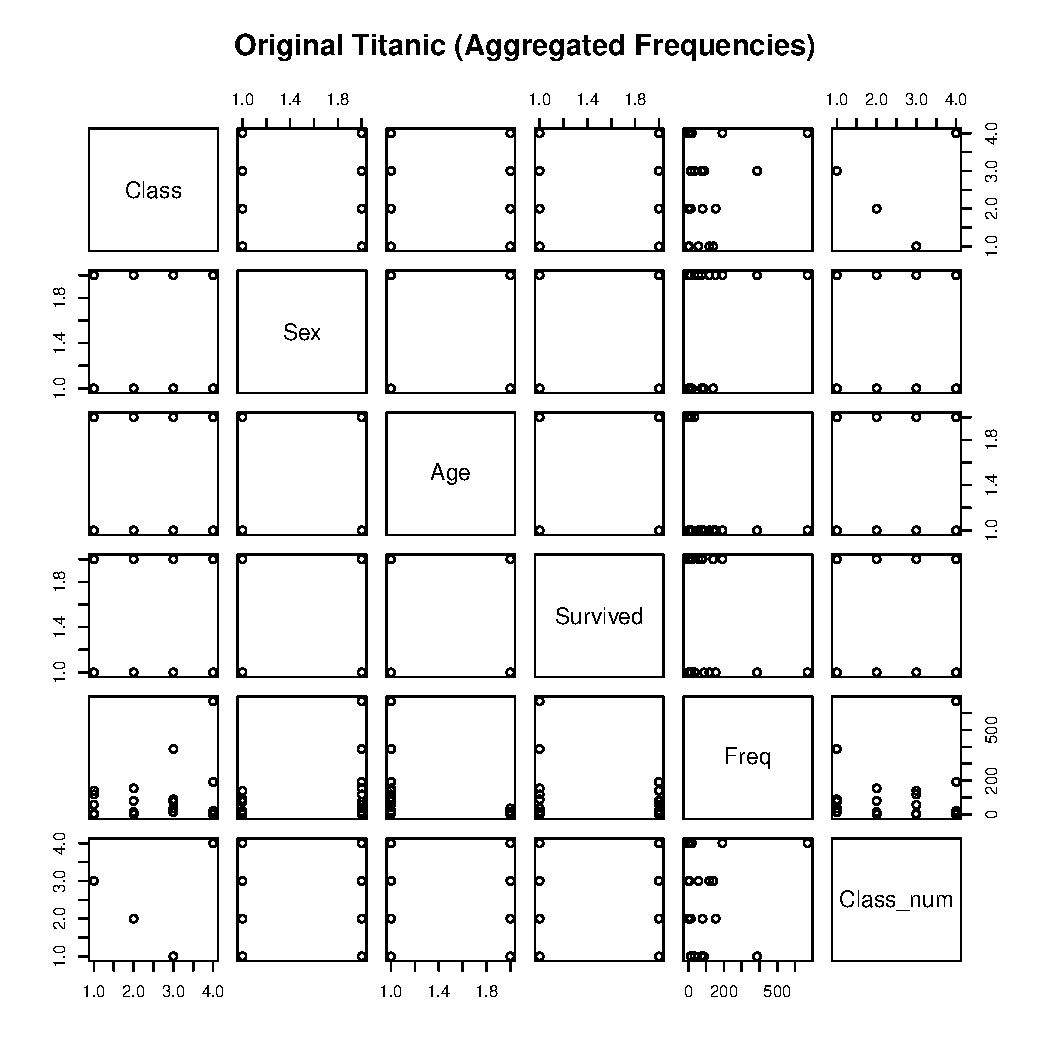
\includegraphics[width=\textwidth]{../dataset/results/plot_titanic_original.pdf}
        \caption{Aggregated Data Plot}
    \end{minipage}\hfill
    \begin{minipage}{0.48\textwidth}
        \centering
        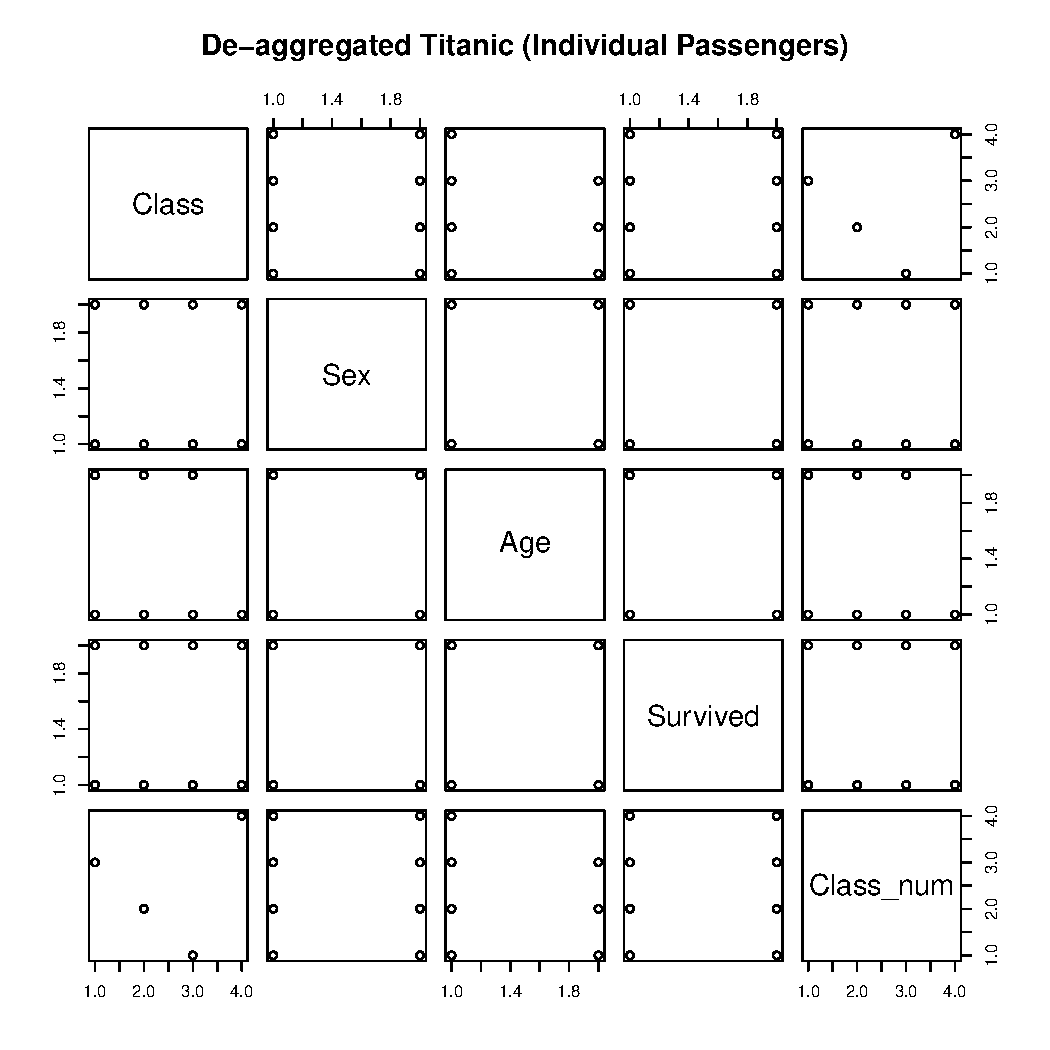
\includegraphics[width=\textwidth]{../dataset/results/plot_titanic2_individual.pdf}
        \caption{Individual Passenger Mosaic}
    \end{minipage}
\end{figure}

The original data frame comprised 32 cross-tabulated contingency records, weighting each profile equally on standard scatter/mosaic plots regardless of frequency. The reconstructed data frame expands into exactly $N=2201$ passenger records. The corresponding mosaic plot accurately displays real demographic imbalances (e.g., substantial crew and 3rd class representation, male majority, and differential survival ratios).

% -------------------------------------------------------------
\section{Exercise 7: Data Selection and Sampling}

\subsection{Correlation Matrices}
Pearson correlation matrices are evaluated using complete pairwise observations.

\begin{lstlisting}[language={}]
> round(cor_air, 3)
         Ozone Solar.R   Wind   Temp  Month    Day
Ozone    1.000   0.348 -0.612  0.699  0.143 -0.005
Solar.R  0.348   1.000 -0.127  0.294 -0.074 -0.058
Wind    -0.612  -0.127  1.000 -0.497 -0.194  0.050
Temp     0.699   0.294 -0.497  1.000  0.404 -0.097
Month    0.143  -0.074 -0.194  0.404  1.000 -0.009
Day     -0.005  -0.058  0.050 -0.097 -0.009  1.000

> round(cor_cars, 3)
      speed  dist
speed 1.000 0.807
dist  0.807 1.000
\end{lstlisting}
\begin{itemize}
    \item \textbf{Redundancy in \texttt{air}:} No pair of attributes satisfies strict redundancy ($|r| \approx 1$). Moderate collinearity exists between \texttt{Temp} and \texttt{Ozone} ($r = 0.699$) and inverse correlation between \texttt{Wind} and \texttt{Ozone} ($r = -0.612$). All variables retain distinct informational value.
    \item \textbf{Redundancy in \texttt{cars}:} A high positive correlation is observed ($r = 0.807$). While stopping distance physically depends on kinetic energy ($\propto v^2$), both attributes measure separate mechanical properties. However, in low-complexity predictive models, this suggests substantial mutual information.
\end{itemize}

\subsection{Sampling Strategies}
\begin{lstlisting}
# Simple random sampling (n = 50)
set.seed(123)
sample_simple <- air[sample(1:nrow(air), size = 50, replace = FALSE), ]
nrow(sample_simple)

# Stratified sampling (5 observations per month)
stratified_idx <- unlist(lapply(split(1:nrow(air), air$Month), function(idx) {
  sample(idx, size = 5, replace = FALSE)
}))
sample_stratified <- air[stratified_idx, ]
table(sample_stratified$Month)
\end{lstlisting}
\begin{lstlisting}[language={}]
> nrow(sample_simple)
[1] 50

> table(sample_stratified$Month)
5 6 7 8 9 
5 5 5 5 5 
\end{lstlisting}
Simple random sampling yields $n=50$ instances drawn uniformly at random. Stratified sampling enforces month-level quota constraints, guaranteeing balanced seasonal representations ($n=25$ total).

% -------------------------------------------------------------
\section{Exercise 8: Data Aggregation}

\subsection{Objective and Commands}
The commercial transactions stored in \texttt{sales-1.txt} are summarized using the \texttt{aggregate()} function across store entities and product categories.

\begin{lstlisting}
sales <- read.table("sales-1.txt", header = TRUE, stringsAsFactors = FALSE)

# Total sales per store
total_sales_store <- aggregate(sales_amount ~ store, data = sales, FUN = sum)

# Average sales per product category
avg_sales_cat <- aggregate(sales_amount ~ product_category, data = sales, FUN = mean)

# Multi-factor aggregation: store and category
total_store_cat <- aggregate(sales_amount ~ store + product_category, data = sales, FUN = sum)

# Bar chart generation and export
pdf("plot_sales_per_store.pdf", width = 6, height = 4.5)
barplot(total_sales_store$sales_amount,
        names.arg = total_sales_store$store,
        col = "steelblue", border = "black",
        main = "Total Sales per Store",
        xlab = "Store Entity", ylab = "Cumulative Sales Amount ($)")
dev.off()
\end{lstlisting}

\subsection{Aggregated Results}
\begin{table}[htbp]
    \centering
    \caption{Summarized Sales Metrics Across Stores and Product Categories}
    \vspace{0.5em}
    \begin{tabular}{llr}
        \toprule
        \textbf{Aggregation Dimension} & \textbf{Level / Group} & \textbf{Metric Value} \\
        \midrule
        Total Sales per Store          & Store\_A               & \$2,430.00            \\
                                       & Store\_B               & \$2,980.00            \\
                                       & Store\_C               & \$1,820.00            \\
        \midrule
        Mean Sales per Category        & Clothing               & \$660.00              \\
                                       & Electronics            & \$1,463.33            \\
                                       & Groceries              & \$430.00              \\
        \bottomrule
    \end{tabular}
\end{table}

\begin{figure}[htbp]
    \centering
    \includegraphics[width=0.55\textwidth]{../dataset/plot_sales_per_store.pdf}
    \caption{Cumulative sales performance broken down by individual retail store.}
\end{figure}

Store\_B generated the highest aggregate revenue (\$2,980), followed by Store\_A (\$2,430) and Store\_C (\$1,820). Across merchandise types, Electronics exhibits the highest mean transaction value (\$1,463.33).

% -------------------------------------------------------------
\section{Exercise 9: Merging Relational Datasets}

\subsection{Objective and Commands}
Relational joining is evaluated by matching customer records from \texttt{customers.txt} against transaction orders in \texttt{orders.txt} along the primary/foreign key \texttt{customer\_id}.

\begin{lstlisting}
# Ingestion
customers <- read.table("customers.txt", header = TRUE, stringsAsFactors = FALSE)
orders    <- read.table("orders.txt", header = TRUE, stringsAsFactors = FALSE)

# Inner join across customer_id
customer_orders <- merge(customers, orders, by = "customer_id", all = FALSE)

# Count of unique matched customers
unique_cust_count <- length(unique(customer_orders$customer_id))

# Total order frequency per customer
orders_per_customer <- table(customer_orders$customer_id)

# Export merged data frame
write.csv(customer_orders, file = "customer_orders.csv", row.names = FALSE)
\end{lstlisting}

\subsection{Discussion}
The inner join operation filters records to preserve only those customer identifiers present simultaneously in both tables. Customer purchase histories are aggregated, quantifying repeat-buyer engagement metrics prior to persisting the consolidated relational view into \texttt{customer\_orders.csv}.

\newpage
\appendix
\section*{Appendix: Complete Execution Log}
\addcontentsline{toc}{section}{Appendix: Complete Execution Log}

The following block contains the verbatim console output generated from running the complete script \texttt{pract2.R} sequentially:

\lstinputlisting[
    language={},
    basicstyle=\ttfamily\tiny,
    frame=single,
    breaklines=true,
    numbers=none,
    title={Console Output: output-pract2.txt}
]{../resultados-pract2.txt}
\end{document}